\documentclass[10pt]{beamer}
\usepackage{ragged2e}
\usepackage{xcolor,colortbl}
\usepackage{hyperref}
\hypersetup{
colorlinks=true,     
urlcolor= red}
\usetheme[
%%% options passed to the outer theme
%    hidetitle,           % hide the (short) title in the sidebar
%    hideauthor,          % hide the (short) author in the sidebar
%    hideinstitute,       % hide the (short) institute in the bottom of the sidebar
%    shownavsym,          % show the navigation symbols
%    width=2cm,           % width of the sidebar (default is 2 cm)
%    hideothersubsections,% hide all subsections but the subsections in the current section
%    hideallsubsections,  % hide all subsections
%    left                % right of left position of sidebar (default is right)
  ]{Aalborg}
  
% If you want to change the colors of the various elements in the theme, edit and uncomment the following lines
% Change the bar and sidebar colors:
%\setbeamercolor{Aalborg}{fg=red!20,bg=red}
%\setbeamercolor{sidebar}{bg=red!20}
% Change the color of the structural elements:
%\setbeamercolor{structure}{fg=red}
% Change the frame title text color:
%\setbeamercolor{frametitle}{fg=blue}
% Change the normal text color background:
%\setbeamercolor{normal text}{bg=gray!10}
% ... and you can of course change a lot more - see the beamer user manual.

\usepackage[utf8]{inputenc}
\usepackage[english]{babel}
\usepackage[sfdefault]{ClearSans}
\usepackage[T1]{fontenc}
%\usepackage{helvet}
\usepackage[scale=1]{ccicons}
\definecolor{gold}{rgb}{0.85,.66,0}
 \definecolor{khaki}{rgb}{0.941176,0.901961,0.549020}
\definecolor{saffron}{rgb}{0.96, 0.77, 0.19}
\definecolor{sand}{rgb}{0.76, 0.7, 0.5}
\definecolor{ablue}{rgb}{0.94, 0.97, 1.0}
\definecolor{cgreen}{rgb}{0.0, 0.42, 0.24}
\setbeamercolor{bgcolor}{fg=black,bg=ablue}
\setbeamercolor{separation line}{use=structure,bg=structure.fg!30!bg}
\setbeamercolor{block body}{fg=black,bg=ablue}

\newenvironment<>{varblock}[2][.9\textwidth]{%
  \setlength{\textwidth}{#1}
  \begin{actionenv}#3%
    \def\insertblocktitle{#2}%
    \par%
    \usebeamertemplate{block begin}}
  {\par%
    \usebeamertemplate{block end}%
  \end{actionenv}}


\setbeamercolor{normal text}{fg=black} 

% colored hyperlinks
\newcommand{\chref}[2]{%
  \href{#1}{{\usebeamercolor[bg]{Aalborg}#2}}%
}

\title[\LaTeX{} Workshop]% optional, use only with long paper titles
{Workshop on ``Document Typesetting and Processing with \LaTeX{}''\vspace{0.2cm}}

\subtitle{\textbf{Session: Cross-Referencing and Hyper-linking}}  % could also be a conference name

\date{\today}

\author[\ccby{} P. K. Yadav \& K. Kumar] % optional, use only with lots of authors
{
  \textbf{P. K. Yadav \& K. Kumar}\\
  \href{mailto:kamal.kumar@jaipur.manipal.edu}{{\tt kamal.kumar@jaipur.manipal.edu}}
}

\institute[
%  {\includegraphics[scale=0.2]{aau_segl}}\\ %insert a company, department or university logo
  Dept.\ of Civil Engineering\\
  Manipal University Jaipur\\
  
] % optional - is placed in the bottom of the sidebar on every slide
{% is placed on the bottom of the title page
  Department of Civil Engineering\\

  

}

% specify the logo in the top right/left of the slide
\pgfdeclareimage[height=1cm]{mainlogo}{fig/mujlogo4} % placed in the upper left/right corner
\logo{\pgfuseimage{mainlogo}}

% specify a logo on the titlepage (you can specify additional logos an include them in 
% institute command below
\pgfdeclareimage[height=2cm]{titlepagelogo}{fig/logofinal} % placed on the title page
%\pgfdeclareimage[height=1.5cm]{titlepagelogo2}{AAUgraphics/aau_logo_new} % placed on the title page
\titlegraphic{% is placed on the bottom of the title page
  \pgfuseimage{titlepagelogo}
%  \hspace{1cm}\pgfuseimage{titlepagelogo2}
}

\begin{document}
% the titlepage
{\aauwavesbg
\begin{frame}[plain,noframenumbering] % the plain option removes the sidebar and header from the title page
  \titlepage
\end{frame}}

% TOC
%\begin{frame}{Agenda}{}
%\tableofcontents
%\end{frame}
%%%%%%%%%%%%%%%%

\section{Motivation}
% motivation for creating this theme
\begin{frame}{Motivation}{}
\begin{block}{}
\justifying
\vspace{0.5cm}
Modern documents include apart from body text, equations, figures, tables, links to the website, and most importantly references. \\
\vspace{0.5cm}

All documents parts are described in the body text, and therefore, they need to be linked. Cross-referencing does this.\\
\vspace{0.5cm}

Documents often are linked with internet links and contain internet related information such as e-mail addresses. These can be linked using hyperlink.\\
\vspace{0.5cm}

Cross-linking is one of the strength of the \LaTeX{} typesetting.

\vspace{0.5cm}
 
\end{block}
\end{frame}

\section{The Label-Ref. thing}

\begin{frame}{The Label$-$Ref. thing I}{}
\begin{block}{The most important specifier \vspace{0.8cm}}
\justifying

\LaTeX{} required only two commands for cross-referencing. They are:\\
\vspace{0.3cm}
\begin{itemize}
\item \textcolor{red}{$\backslash$label\{key\}}, where \textbf{``key''} is identifier, which could be any text or text and number.\\
\vspace{0.3cm}

\item \textcolor{red}{$\backslash$ref\{key\}}, where the  \textbf{``key''} must be identical to the key used with \textbf{label} specifier.\\

\end{itemize}
\vspace{0.3cm}
Let us check that in an example.

\end{block}
\end{frame}

\begin{frame}[fragile]{The Link$-$Ref. thing II}{}
\begin{block}{A Example}



\justifying

    \begin{beamercolorbox}[rounded=true, center, shadow=true,wd=9cm]{bgcolor}
    \vspace{-0.5cm}
      \begin{verbatim}
   \section{Greetings}\label{sec:greetings}
      Hello! welcome to \LaTeX{} workshop.
    
   \section{Referencing}
      I greeted in section~\ref{sec:greetings}.
           \end{verbatim}
           \vspace{-0.6cm}
    \end{beamercolorbox}
    
    
Results to:\\
\vspace{0.3cm}

 \begin{beamercolorbox}[rounded=true, center, shadow=true,wd=8cm, colsep=1.5pt]{upper separation line foot}
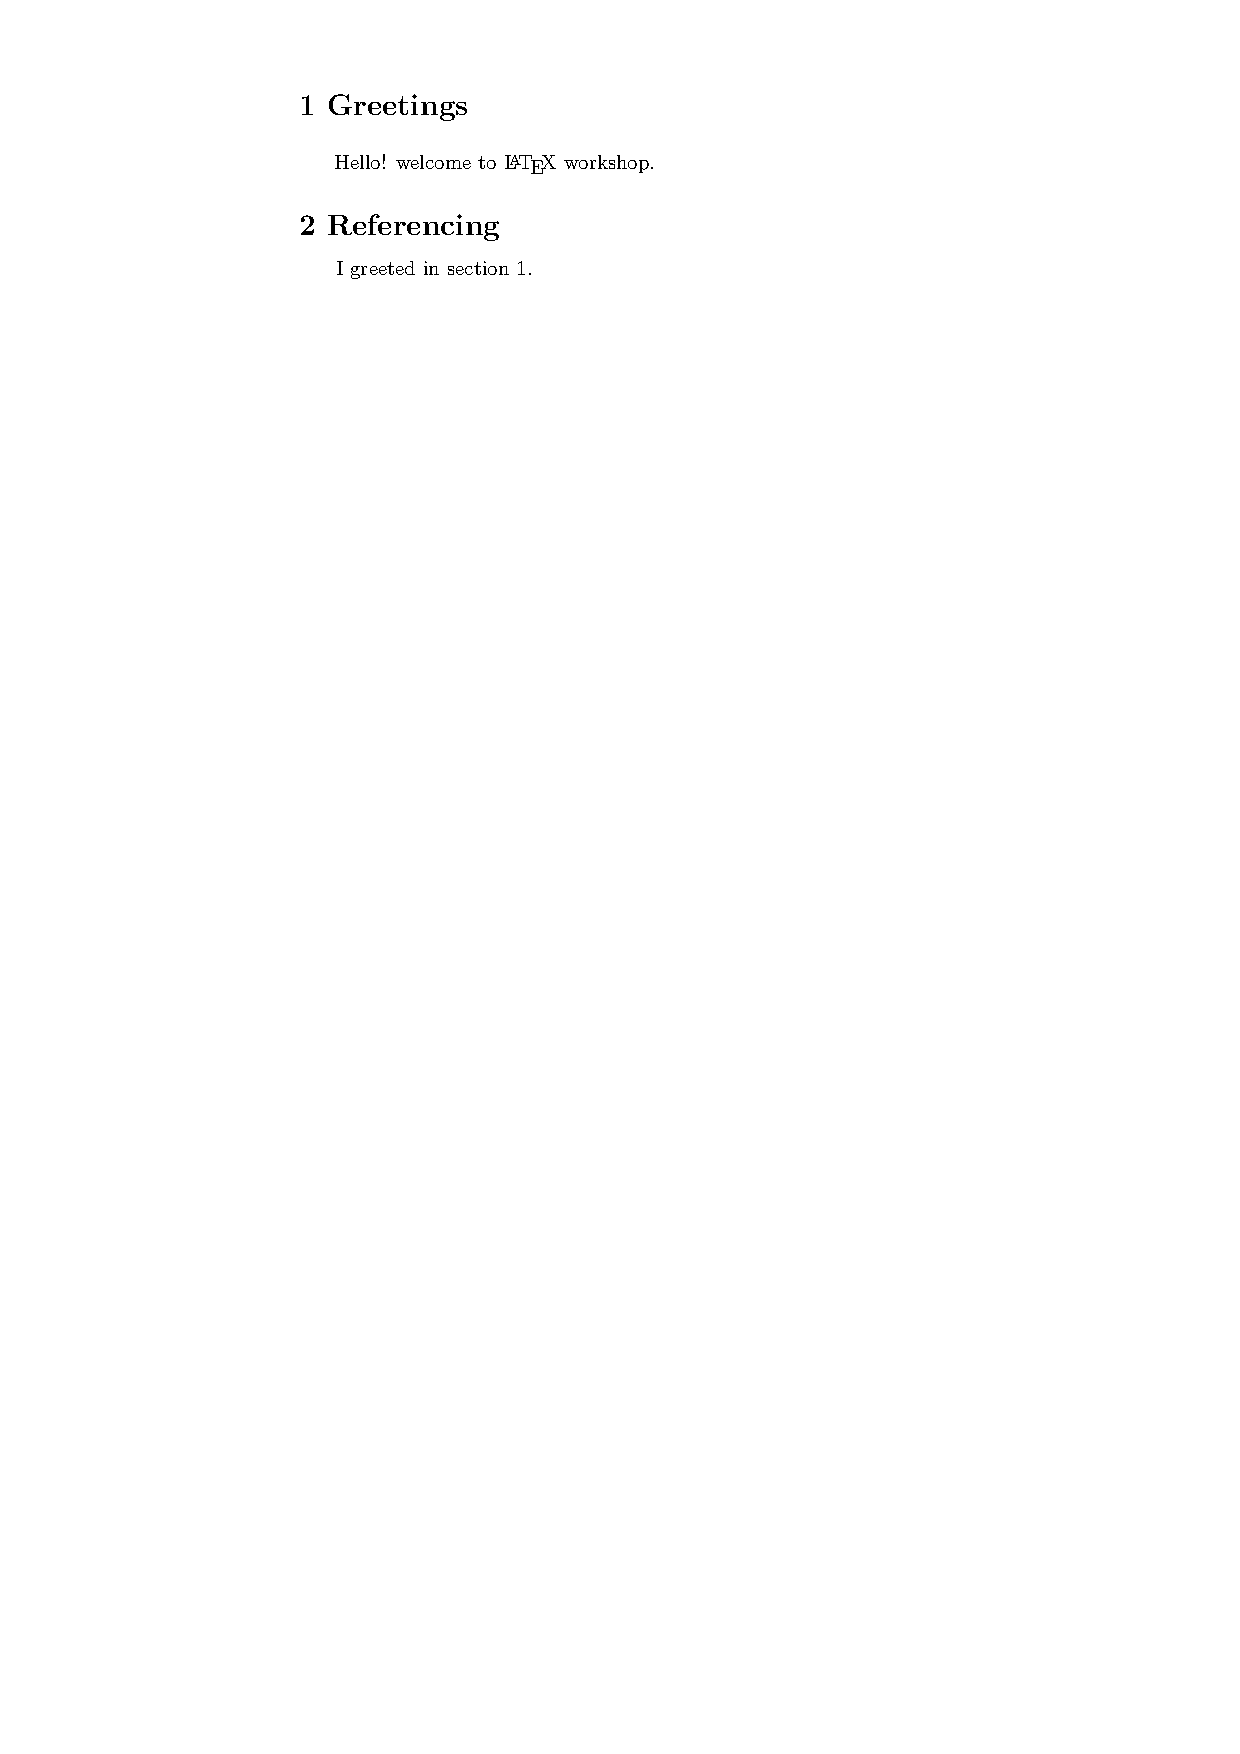
\includegraphics[width = 6cm]{fig/fig3}
    \end{beamercolorbox}

\end{block}
\end{frame}

\begin{frame}[fragile]{The Link$-$Ref. thing III}{}
\begin{block}{Positioning the \textcolor{red}{$\backslash$label\{key\}} \vspace{0.4cm}}



\justifying

The \textcolor{red}{$\backslash$label\{key\}} can be placed anywhere, in principle,and then be referred. Some exceptional are:\\

\vspace{0.3 cm}
\begin{enumerate}

\item In \textbf{figure} and \textbf{table} environments, \textcolor{red}{$\backslash$label\{key\}} has to be placed after (or inside) the \textcolor{red}{$\backslash$caption\{ \}} specifier in order to get the correct referring.\\

\vspace{0.3 cm}

\item In the \textbf{equation} environment \textcolor{red}{$\backslash$label\{key\}} is placed just after the \textcolor{red}{$\backslash$begin\{equation\}} specifier, e.g.\\

\end{enumerate}

  \begin{beamercolorbox}[rounded=true, center, shadow=true,wd=7cm, colsep=1.5pt]{upper separation line foot}
     \vspace{-0.5cm}
       \begin{verbatim}
    \begin{equation} \label{eq:solve}
    x^2 - 5 x + 6 = 0
    \end{equation}
            \end{verbatim}
            \vspace{-0.6cm}
     \end{beamercolorbox}
     
     

\end{block}
\end{frame}

\section{Useful Packages}
\begin{frame}[fragile]{Useful Packages I}{}
\begin{block}{The amsmath package\vspace{0.2cm}}


\justifying


The \textbf{amsmath} package provide the following four very useful specifier:

\begin{enumerate}

\item The \textcolor{red}{$\backslash$eqref\{ \}} specifier, which adds brackets so that, instead of printing a plain number as 5, it will print (5).\\
\vspace{0.3cm}

\item The \textcolor{red}{$\backslash$tag{eqno}} sets eqno can be any arbitrary string specifying the equation number.\\
\vspace{0.3cm}


\item The \textcolor{red}{$\backslash$numberwithin\{equation\}\{section\}} adds section numbers to the eqaution number.

\end{enumerate}

\end{block}
\end{frame}

\begin{frame}[fragile]{Useful Packages II}{}
\begin{block}{The hyperref package\vspace{0.4cm}}


\justifying


The package \textbf{hyperref} provides LaTeX the ability to create hyperlinks within the document. Once loaded, the possibility to include interactive external links and all internal references turns to hyperlinks.\\
\vspace{0.2cm}

The hyperref package is loaded in preamble as:\\ $\backslash$usepackage\{hyperref\}.\\
\vspace{0.2cm}

Among the most useful hyperref commands are:

\begin{itemize}
\item The \verb|\href{my_url}{<description>}|; e.g. \href{www.sharda.ac.in}{Sharda University}\\
\vspace{0.2cm}

\item The \verb|\href{mailto:mailme@email.com}{mailme@eamil.com}| provides the possibility to link your document to email address. e.g. \href{mailto:ruban.sugumar@sharda.ac.in}{ruban.sugumar@sharda.ac.in}
\end{itemize}

\end{block}
\end{frame}

\section{End Remarks}
\begin{frame}[fragile]{End Reamarks}{}
\begin{block}{}

\justifying
Cross-referencing in \LaTeX{} is simple and very extensive. Several additional packages further extends cross-referencing within and to the internet. Following references can be used for advancing knowledge.\\
\vspace{0.2cm}



\begin{itemize}

\item The hyperref package is very extensible, detail can be found \href{http://en.wikibooks.org/wiki/LaTeX/Hyperlinks}{here}.\\
\vspace{0.2cm}

\item Some addition packages for cross-referencing are: \href{http://www.ctan.org/pkg/varioref}{varioref, for page referencing}, \href{http://www.ctan.org/pkg/nameref}{nameref, for section naming}, \href{http://www.ctan.org/pkg/cleveref}{intelligent cross-referencing} etc.\\
\vspace{0.2cm}

\item Good tutorial on cross-referencing can be found \href{http://www.tug.org/tutorials/tugindia/chap12-scr.pdf}{here} and \href{http://en.wikibooks.org/wiki/LaTeX/Labels_and_Cross-referencing#tag}{here}.\\
\vspace{0.2cm}

\end{itemize} 


\end{block}
\end{frame}

{\aauwavesbg%
\begin{frame}[plain,noframenumbering]%
  \finalpage{\huge Thank you for your participation\\ \vspace{0.3cm}\textbf{ We wish you a good time with \LaTeX{}!}}
\end{frame}}


\end{document}
